% D.23 圆内接四边形 ABCD
\documentclass[tikz,border=4pt]{standalone}
\usepackage{ctex}
\usepackage{amsmath}
\usetikzlibrary{calc}
\begin{document}
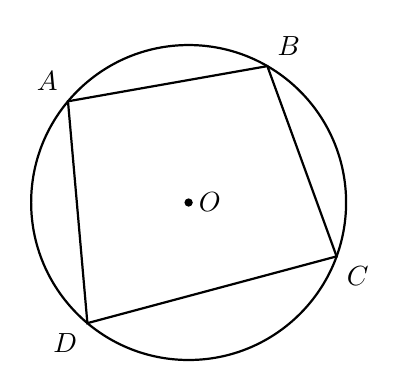
\begin{tikzpicture}[scale=1.0, thick]
  \coordinate (O) at (0, 0);
  \draw (O) circle (2);
  \coordinate (A) at ({2*cos(140)}, {2*sin(140)});
  \coordinate (B) at ({2*cos( 60)}, {2*sin( 60)});
  \coordinate (C) at ({2*cos(-20)}, {2*sin(-20)});
  \coordinate (D) at ({2*cos(-130)}, {2*sin(-130)});

  \draw (A) -- (B) -- (C) -- (D) -- cycle;
  \fill (O) circle (1.5pt);
  \node[right] at (O) {$O$};
  \node[above left]  at (A) {$A$};
  \node[above right] at (B) {$B$};
  \node[below right] at (C) {$C$};
  \node[below left]  at (D) {$D$};
\end{tikzpicture}
\end{document}
